% !TEX TS-program = xelatex
% !TeX document-id = {c6282027-a510-40f1-b05e-2f558a6cd3f1}
% !TeX program = xelatex
% !TeX TXS-program:compile = txs:///xelatex/[--shell-escape]
%%%%%%%%%%%%%%%%%%%%%%%%%%%%%%%%%%%%%%%%%%%%%%%%%%%%%%%%%%%%%%%%%%%%%%%%
% Plantilla TFG/TFM
% Universidad de Murcia. Facultad de Informática
% Realizado por: José Manuel Requena Plens
% Modificado: Pablo José Rocamora Zamora
% Contacto: pablojoserocamora@gmail.com
%%%%%%%%%%%%%%%%%%%%%%%%%%%%%%%%%%%%%%%%%%%%%%%%%%%%%%%%%%%%%%%%%%%%%%%%


% Archivo .TEX que incluye todas las configuraciones del documento y los paquetes. Añade todo aquello que necesites utilizar en el documento en este archivo.
% En él se encuentra la configuración de los márgenes, establecidos según las directrices de estilo de la EPS.
\input{include/configuracioninicial}

%%%%%%%%%%%%%%%%%%%%%%%%%%%%%%%%%%%%%%%%%%%%%%%%%%%%%%%%%%%%%%%%%%%%%%
% INFORMACIÓN DEL TFG
% Comentar lo que NO se desee añadir y sustituir con la información correcta.
%%%%%%%%%%%%%%%%%%%%%%%%%%%%%%%%%%%%%%%%%%%%%%%%%%%%%%%%%%%%%%%%%%%%%%
% Título y subtítulo
\newcommand{\titulo}{MMT Chat}
\newcommand{\subtitulo}{Creación de un chatbot con IA capaz de buscar información en fuentes externas}
% Datos del autor
\newcommand{\miNombre}{Mario Martínez Turpín}
\newcommand{\miDNI}{49183039T}
\newcommand{\miEmail}{m.martinezturpin@um.es}
% Datos del tutor/es
\newcommand{\miTutor}{Jose Antonio Miñarro Gimenez (tutor1)}
\newcommand{\miTutorB}{Catalina Martínez Costa (tutor2)}
\newcommand{\departamentoTutor}{Departamento de Informática y Sistemas}
% Datos de la facultada y universidad
\newcommand{\miFacultad}{Facultad de Informática}
\newcommand{\miFacultadCorto}{FIUM}
\newcommand{\miUniversidad}{\protect{Universidad de Murcia}}
\newcommand{\miUbicacion}{Murcia}
\newcommand{\firma}{include/firma}

% Configuración automática según el identificador elegido
% Grados
\definecolor{informatica}{RGB}{121,11,21}	% Informatica
% Colores generales
\definecolor{negro}{RGB}{0,0,0}
\definecolor{blanco}{RGB}{255,255,255}

% Logotipos comunes de todas las titulaciones
\newcommand{\logoFacultadPortada}{include/logos-titulaciones/Simbolo-negativo-sin-fondo}
\newcommand{\logoGradoPortada}{include/logos-titulaciones/Simbolo-negativo-sin-fondo} 
\newcommand{\logoUniversidadPortada}{include/logos-universidad/escudo_umu}
\newcommand{\logoFacultadPortadaBaja}{include/logos-titulaciones/FIUM-postivo-sin-fondo}
% Logos
\newcommand{\logoGrado}{include/logos-titulaciones/FI-positivo}
\newcommand{\logoDepartamento}{include/logos-titulaciones/Logotipo_DIIC}
\newcommand{\logoUniversidad}{include/logos-universidad/um}
% Texto
\newcommand{\miGrado}{Grado en Ingeniería Informática}
\newcommand{\tipotrabajo}{Trabajo Fin de Grado}
% Color
\newcommand{\colorgrado}{informatica}
\newcommand{\colortexto}{blanco}

% Información añadida a las propiedades del archivo PDF.
\hypersetup{
	pdfauthor = {\miNombre~(\miEmail)},
	pdftitle = {\titulo},
}

%%
% Archivo de acrónimos
%%
\makeglossaries% Genera la base de datos de acrónimos
%%%%%%%%%%%%%%%%%%%%%%%%%%%%%%%%%%%%%%%%%%%%%%%%%%%%%%%%%%%%%%%%%%%%%%%%
% Plantilla TFG/TFM
% Universidad de Murcia. Facultad de Informática
% Realizado por: José Manuel Requena Plens
% Modificado: Pablo José Rocamora Zamora
% Contacto: pablojoserocamora@gmail.com
%%%%%%%%%%%%%%%%%%%%%%%%%%%%%%%%%%%%%%%%%%%%%%%%%%%%%%%%%%%%%%%%%%%%%%%%


% Lista de acrónimos (se ordenan por orden alfabético automáticamente)

% La forma de definir un acrónimo es la siguiente:
% \newacronyn{id}{siglas}{descripción}
% Donde:
% 	'id' es como vas a llamarlo desde el documento.
%	'siglas' son las siglas del acrónimo.
%	'descripción' es el texto que representan las siglas.
%
% Para usarlo en el documento tienes 4 formas:
% \gls{id} - Añade el acrónimo en su forma larga y con las siglas si es la primera vez que se utiliza, el resto de veces solo añade las siglas. (No utilices este en títulos de capítulos o secciones).
% \glsentryshort{id} - Añade solo las siglas de la id
% \glsentrylong{id} - Añade solo la descripción de la id
% \glsentryfull{id} - Añade tanto  la descripción como las siglas

\newacronym{api}{API}{Application Programming Interface}
\newacronym{kg}{KG}{Knowledge Graph}
\newacronym{llm}{LLM}{Large Language Model}
\newacronym{json}{JSON}{JavaScript Object Notation}
\newacronym{nt}{NT}{N-Triples}
\newacronym{nlp}{NLP}{Natural Language Processing}
\newacronym{pln}{PLN}{Procesamiento de Lenguaje Natural}
\newacronym{rag}{RAG}{Retrieval-Augmented Generation}
\newacronym{rdf}{RDF}{Resource Description Framework}
\newacronym{sparql}{SPARQL}{Simple Protocol and RDF Query Language}
\newacronym{ui}{UI}{User Interface}
 % Archivo que contiene los acrónimos

%%%%%%%%%%%%%%%%%%%%%%%% 
% INICIO DEL DOCUMENTO
% A partir de aquí debes empezar a realizar tu TFG/TFM
%%%%%%%%%%%%%%%%%%%%%%%%
\begin{document}
	
	% Números romanos hasta el mainmatter.
	\frontmatter
	
	% PORTADA
	\input{include/portada/portada_color} % Portada Color
	%\input{include/portada/portada_bn} % Portada B/N
	
	%%%%% PREAMBULO
	% Incluye el .tex que contiene el preámbulo, agradecimientos y dedicatorias.
	%\setstretch{1.5} % 1.5 línea de interlineado antes esta a 1 para la portada
	%%%%%%%%%%%%%%%%%%%%%%%%%%%%%%%%%%%%%%%%%%%%%%%%%%%%%%%%%%%%%%%%%%%%%%%%
% Plantilla TFG/TFM
% Universidad de Murcia. Facultad de Informática
% Realizado por: José Manuel Requena Plens
% Modificado: Pablo José Rocamora Zamora
% Contacto: pablojoserocamora@gmail.com
%%%%%%%%%%%%%%%%%%%%%%%%%%%%%%%%%%%%%%%%%%%%%%%%%%%%%%%%%%%%%%%%%%%%%%%%




\cleardoublepage %salta a nueva página impar

\chapter*{Agradecimientos
}

\thispagestyle{empty}
\vspace{1cm}

Me gustaría expresar mi agradecimiento a mis tutores, Jose Antonio Miñarro Gimenez y Catalina Martínez Costa, por su guía a lo largo de todo el proceso. Su ayuda ha sido fundamental para navegar los procedimientos formales y darle forma al trabajo.\bigskip

Asimismo, quiero agradecer a mi familia por el apoyo incondicional y la confianza que han depositado en mí durante todo este tiempo. Sin ellos, este proyecto no habría sido posible.


También quiero destacar a mi pareja, Natalia, por su amor, paciencia y comprensión, que tanto me han ayudado a seguir adelante durante estos meses.\bigskip

Finalmente, dedico este trabajo a todas las personas que han contribuido a que esta experiencia sea enriquecedora y exitosa. Su ayuda y confianza me han permitido alcanzar
mis objetivos y convertir esta tesis en una realidad.

\cleardoublepage %salta a nueva página impar

% Aquí va la dedicatoria si la hubiese. Si no, comentar la(s) linea(s) siguientes
%\chapter*{}
%\setlength{\leftmargin}{0.5\textwidth}
%\setlength{\parsep}{0cm}
%\addtolength{\topsep}{0.5cm}

%\begin{flushright}
%	\small\em{
%		A mi esposa Marganit, y a mis hijos Ella Rose y Daniel Adams,\\
%		sin los cuales habría podido acabar este libro dos años antes \footnote{Dedicatoria de Joseph J. Roman en "An Introduction to Algebraic Topology"}
%	}
%\end{flushright}


\cleardoublepage %salta a nueva página impar

% Aquí va la cita célebre si la hubiese. Si no, comentar la(s) linea(s) siguientes
%\chapter*{}

%\setlength{\leftmargin}{0.5\textwidth}
%\setlength{\parsep}{0cm}
%\addtolength{\topsep}{0.5cm}
%\begin{flushright}
%	\small\em{
%		Si consigo ver más lejos\\
%		es porque he conseguido auparme\\ 
%		a hombros de gigantes
%	}
%\end{flushright}

%\begin{flushright}
%	\small{
%		Isaac Newton.
%	}
%\end{flushright}

\cleardoublepage %salta a nueva página impar


	\input{preambulos/1_declaracion_originalidad}
	%%%%%%%%%%%%%%%%%%%%%%%%%%%%%%%%%%%%%%%%%%%%%%%%%%%%%%%%%%%%%%%%%%%%%%%%
% Plantilla TFG/TFM
% Universidad de Murcia. Facultad de Informática
%%%%%%%%%%%%%%%%%%%%%%%%%%%%%%%%%%%%%%%%%%%%%%%%%%%%%%%%%%%%%%%%%%%%%%%%


\chapter*{Resumen}

En la era digital actual, el acceso eficiente y preciso a grandes volúmenes de información estructurada y no estructurada representa uno de los mayores desafíos en el ámbito de las Ciencias de la Computación. Históricamente, la Web Semántica y los Grafos de Conocimiento (\textit{Knowledge Graphs}) han proporcionado un marco tecnológico robusto para modelar información de manera determinista mediante tripletas (Sujeto, Predicado, Objeto) basadas en el estándar RDF (Resource Description Framework). El acceso a esta información altamente estructurada y veraz se realiza tradicionalmente a través de SPARQL, un lenguaje de consulta potente pero con una curva de aprendizaje pronunciada que supone una barrera técnica insalvable para la mayoría de los usuarios no expertos.

De forma paralela, el reciente auge de los Modelos de Lenguaje de Gran Escala (LLMs) ha revolucionado la interacción humano-máquina. Estos modelos permiten establecer interfaces conversacionales fluidas en lenguaje natural, facilitando enormemente el acceso a la información. Sin embargo, su naturaleza estocástica los hace vulnerables a problemas inherentes como las denominadas "alucinaciones" (la generación de respuestas que resultan gramaticalmente correctas y plausibles, pero que son total o parcialmente falsas) y presentan serias dificultades para recuperar datos precisos y actualizados de dominios de conocimiento altamente específicos.

El presente Trabajo de Fin de Grado (TFG) aborda la convergencia de ambas tecnologías con el objetivo de aunar la flexibilidad y capacidad de comprensión del lenguaje natural propia de los LLMs con la precisión factual inmutable de un Grafo de Conocimiento. Para lograr este ambicioso objetivo, se ha diseñado, implementado y evaluado un agente conversacional inteligente (chatbot) especializado en el dominio cinematográfico. A diferencia de un chatbot tradicional que responde basándose puramente en los patrones aprendidos en su entrenamiento, este sistema actúa como una interfaz transparente que traduce la intención del usuario a consultas SPARQL válidas, ejecutándolas contra una base de datos local y devolviendo la respuesta exacta.

La arquitectura del sistema propuesto se fundamenta en una evolución del paradigma de Generación Aumentada por Recuperación (RAG), elevándolo hacia un sistema de Inteligencia Artificial Agéntica. La solución tecnológica se ha estructurado en tres capas principales. En la capa de presentación, se ha desarrollado una interfaz gráfica de usuario amigable mediante Streamlit, que no solo facilita la interacción conversacional, sino que también expone de manera transparente el razonamiento interno del agente ("Chain-of-Thought") y las consultas generadas en tiempo real. En la capa lógica, el núcleo cognitivo del sistema, impulsado por el modelo Llama 3 ejecutado localmente mediante Ollama, se encarga de la extracción de entidades, su desambiguación contra el vocabulario de Wikidata y la generación dinámica de código SPARQL. Finalmente, la capa de datos descansa sobre un Grafo de Conocimiento local alojado en el motor de base de datos Blazegraph.

Un hito técnico fundamental de este trabajo ha sido la construcción de este repositorio de datos semántico. Depender directamente de \textit{endpoints} públicos como el de Wikidata durante la ejecución en tiempo real introducía niveles inaceptables de latencia y riesgo de bloqueos por límites de peticiones (APIs \textit{rate limits}). Por ello, se implementó un proceso de extracción \textit{offline} estructurado para aislar un subgrafo densamente conectado del dominio cinematográfico (abarcando miles de películas, directores, actores, géneros y fechas de estreno), el cual fue serializado e indexado localmente. Esto proporciona al agente un entorno de ejecución local, excepcionalmente rápido y completamente determinista.

El aspecto más innovador de la implementación radica en el mecanismo autónomo de autocorrección del agente, denominado "bucle de reflexión" (\textit{Reflexion Loop}). La traducción de lenguaje natural a sintaxis SPARQL estricta es propensa a errores. Para mitigarlo, el agente cuenta con un diccionario de propiedades permitidas altamente restrictivo (por ejemplo, \texttt{wdt:P57} exclusivamente para referenciar a un "director") que acota drásticamente su espacio de búsqueda. Si el modelo genera una consulta con errores de sintaxis o que no compila, la capa de datos captura la excepción y, en lugar de fallar de manera abrupta, realimenta al LLM con este error inyectado en un \textit{prompt} de reflexión. De este modo, el agente analiza lógicamente su propia equivocación y reescribe la consulta desde cero, logrando un notable incremento en la robustez, resiliencia y autonomía del sistema.

Para validar el sistema propuesto de forma objetiva, rigurosa y cuantitativa, se desarrolló ad-hoc un marco de evaluación automatizado. Se confeccionó un conjunto de pruebas (\textit{dataset}) compuesto por 103 consultas complejas en lenguaje natural que abarcaban diversas relaciones semánticas de dificultad incremental. El entorno de evaluación puso a prueba seis modelos LLM locales diferentes (Llama 3, Llama 3.2:1B, Mistral, Gemma 2:9B, Gemma 2:2B y DeepSeek-R1:8B) para analizar su rendimiento de forma comparativa. El modelo seleccionado para la versión final del proyecto, Llama 3, demostró un rendimiento excepcional: alcanzó una tasa de precisión del 97.1\% en la fase crítica de extracción de entidades, un 97.1\% en la generación de código SPARQL válido y ejecutable, y un porcentaje de éxito final del 94.3\% entregando la respuesta correcta a la pregunta planteada.

Además de las tasas de éxito en precisión, se midió exhaustivamente el tiempo de ejecución por pregunta, un factor sumamente crítico para asegurar una buena experiencia de usuario en cualquier asistente conversacional interactivo. Llama 3 demostró un rendimiento óptimo en este aspecto, promediando un tiempo de ejecución de respuesta de tan solo 9.51 segundos por pregunta, erigiéndose de manera destacada como el modelo más equilibrado y rápido de entre todos los evaluados en este trabajo. Un análisis pormenorizado de los escasos fallos residuales reveló que estos se debían, en su inmensa mayoría, a ambigüedades idiomáticas extremas por parte del usuario o a cuellos de botella aislados en las llamadas de desambiguación de entidades, y no a fallos estructurales o lógicos en la formulación de consultas deductivas por parte del LLM.

En conclusión, los resultados empíricos obtenidos a lo largo de las pruebas confirman sin lugar a dudas que la integración de agentes de IA fuertemente tipados con Grafos de Conocimiento locales constituye una solución tecnológica sumamente viable y efectiva para la creación de sistemas de pregunta-respuesta (QA) totalmente transparentes y estructuralmente libres de alucinaciones. El sistema diseñado ha logrado el hito de ocultar la enorme complejidad inherente al modelo de datos de la Web Semántica de cara al usuario final, manteniendo no obstante intacta la rigurosa precisión y veracidad de sus datos subyacentes. El presente trabajo sienta, por tanto, unas bases sólidas y prometedoras para futuras líneas de investigación y desarrollo, tales como la mejora de los algoritmos basados en similitud de vectores (\textit{embeddings}) para lograr una desambiguación semántica libre de fallos, o la ampliación escalonada de la ontología base para llegar a soportar razonamientos deductivos mucho más complejos de múltiples saltos lógicos (\textit{multi-hop reasoning}) que permitan extraer conclusiones de datos aparentemente inconexos.

\vspace{1cm}
\textbf{Palabras clave:} Web Semántica, Grafos de Conocimiento, SPARQL, Modelos de Lenguaje (LLMs), Llama3, Generación Aumentada por Recuperación (RAG), Inteligencia Artificial Agéntica, Streamlit, Blazegraph, Mitigación de Alucinaciones.

	%%%%%%%%%%%%%%%%%%%%%%%%%%%%%%%%%%%%%%%%%%%%%%%%%%%%%%%%%%%%%%%%%%%%%%%%
% Plantilla TFG/TFM
% Universidad de Murcia. Facultad de Informática
%%%%%%%%%%%%%%%%%%%%%%%%%%%%%%%%%%%%%%%%%%%%%%%%%%%%%%%%%%%%%%%%%%%%%%%%


\chapter*{Extended Abstract}

This Final Degree Project presents the comprehensive design, implementation, and rigorous evaluation of an intelligent conversational agent specialized in the cinematographic domain. The primary objective is to bridge the significant technical gap between the natural language comprehension capabilities of modern Large Language Models (LLMs) and the factual, deterministic precision inherent to Semantic Web Knowledge Graphs. By synergizing these two distinct technological paradigms, the project directly addresses one of the most critical and widely discussed challenges in modern generative Artificial Intelligence: the mitigation and elimination of "hallucinations"—the generation of plausible yet entirely fabricated information.

\section*{1. Introduction and Motivation}
In recent years, LLMs have revolutionized the way users and developers interact with information systems, enabling highly fluent conversational interfaces. However, their stochastic nature makes them inherently unreliable for querying specific, factual, or specialized data, as they are prone to generating incorrect answers with high confidence. On the other hand, Knowledge Graphs and the Semantic Web provide impeccably structured, verifiable data environments accessible via precise query languages like SPARQL. The steep learning curve and strict syntax of SPARQL prevent non-expert users from accessing this immense wealth of information. This project proposes a robust hybrid solution: an autonomous conversational agent that acts as a transparent natural language interface for a local Knowledge Graph, intelligently translating user queries into SPARQL, executing them locally, and returning the exact data in a human-readable format.

\section*{2. State of the Art}
The theoretical foundation of this work rests firmly on three technological pillars: the Semantic Web, Large Language Models, and Retrieval-Augmented Generation (RAG) paradigms. The Semantic Web, formalized and standardized by the W3C, relies heavily on the Resource Description Framework (RDF) to elegantly model complex information as subject-predicate-object triples. Wikidata, a massive, multilingual, and collaborative knowledge base, serves as the primary and authoritative data source for this project.

To effectively overcome the static knowledge limitations and hallucination issues of standard LLMs, RAG architectures dynamically retrieve external data and inject it into the model's contextual window. This project pushes the traditional RAG paradigm significantly further by implementing an "Agentic AI" workflow using the LangChain framework. Within this architecture, the LLM is not relegated to merely retrieving text; it actively reasons, plans, writes code, tests queries against the database, and refines its approach.

\section*{3. System Architecture and Methodology}
Given the highly experimental and empirical nature of advanced prompt engineering, an agile, iterative, and test-driven methodology was adopted throughout the development lifecycle. The overall system architecture is modularly divided into three highly cohesive main layers:
\begin{itemize}
    \item \textbf{Presentation Layer:} A highly interactive and responsive graphical user interface built entirely with Streamlit. It provides a seamless chat-like experience while simultaneously displaying the internal reasoning process (Chain-of-Thought) and the generated SPARQL code to the user, ensuring maximum transparency.
    \item \textbf{Logic and Agent Layer:} The cognitive core of the application, powered by LangChain and Llama3 running locally via Ollama. This layer handles the complex tasks of natural language understanding, entity extraction, Wikidata term disambiguation, and the core iterative SPARQL generation loop.
    \item \textbf{Data Layer:} A highly optimized, in-memory RDF local repository serialized in \texttt{.ttl} format, managed by the RDFLib Python library. It contains a densely populated subset of domain-specific cinematic data.
\end{itemize}

\section*{4. Local Knowledge Graph Construction}
Relying directly on public SPARQL endpoints (such as the Wikidata Query Service) during real-time user interaction introduces unacceptable latency and severe risks of being blocked by strict API rate limits. Therefore, a custom, highly tailored data extraction pipeline was developed. The system programmatically queries Wikidata entirely offline to extract a densely connected, self-contained subgraph focusing specifically on movies, directors, actors, genres, and release dates. This data is then serialized into the \textit{Turtle} format. This approach provides a lightning-fast, secure, and fully controlled environment for the agent to execute queries without relying on unstable external network dependencies.

\section*{5. The Reflexion Loop}
Arguably the most innovative and impactful aspect of the system's implementation is the agent's autonomous, self-healing error-correction mechanism. Translating fluid natural language into strict, unforgiving SPARQL syntax is a heavily error-prone task for any LLM. To guide the model, the agent is provided with a strict, curated dictionary of allowed RDF properties (e.g., \texttt{wdt:P57} exclusively for "director"). 

When the agent confidently generates a SPARQL query, the Logic Layer attempts to execute it locally against the Data Layer via RDFLib. If a syntax or execution error occurs, the process does not fail catastrophically. Instead, the runtime traceback is intercepted, parsed, and fed back to the LLM in a specialized "reflexion prompt". This prompt instructs the model to critically analyze its own previous mistake, understand the syntax error, and autonomously rewrite the query. This iterative self-correction loop drastically increases the overall robustness, reliability, and success rate of the system.

\section*{6. Evaluation and Results}
To quantitatively validate the system's performance and viability, a comprehensive automated evaluation framework was built. A rigorous dataset of 61 complex natural language queries was carefully created, covering a wide array of semantic relationships and designed specifically to compare the performance of various large language models. The chosen baseline model for this project (Llama3) achieved an outstanding 90.16\% accuracy rate in the crucial steps of entity extraction and disambiguation. Furthermore, it also achieved a 90.16\% overall success rate in generating valid, executable SPARQL queries that returned the factually correct answer.

Within this framework, we also rigorously evaluated the execution latency per question. Llama3 demonstrated its ideal suitability for real-time conversational AI applications by achieving a remarkable average execution time of just 3.66 seconds per question, which was comfortably the lowest latency among all the sophisticated models tested.

An in-depth analysis of the remaining failure cases revealed that most issues stemmed from extreme idiomatic ambiguities in the user's phrasing or minor, residual API rate limits encountered during the entity disambiguation phase, rather than fundamental logical reasoning failures by the LLM itself. The extraordinarily high success rate in autonomous query generation conclusively proves that heavily constraining the LLM's vast search space through strict prompt engineering and predefined property dictionaries is a highly effective, production-ready strategy.

\section*{7. Conclusions}
The empirical results confirm beyond doubt that integrating powerful LangChain agents with strongly-typed, local Knowledge Graphs is a highly viable and superior technical solution for building transparent, hallucination-free Question-Answering systems. The resulting agentic workflow successfully and completely hid the underlying complexity of the Semantic Web from the end-user, all while retaining and leveraging its absolute factual precision. Future work will strategically focus on improving the semantic similarity algorithms to ensure flawless entity disambiguation, and expanding the underlying ontology to comfortably support highly complex, multi-hop reasoning questions.

\vspace{1cm}
\textbf{Keywords:} Semantic Web, Knowledge Graphs, SPARQL, Large Language Models, Llama3, RAG, LangChain, Agentic AI, Hallucination Mitigation, Streamlit.

	
	%\setstretch{1.0} % 1.0 línea de interlineado para los indices
	% Incluye después del archivo anterior el indice y lista de figuras, tablas y códigos.

	% Modificar el espacio superior a partir de los índices y para el resto de capítulos
	\renewcommand*{\chapterheadstartvskip}{\vspace*{-2cm}}

	\tableofcontents     	%Índice
	\listoffigures	     	%Índice de figuras
	\listoftables	     	%Índice de tablas
	\lstlistoflistings%Índice de códigos
	
	% Inicia la numeración habitual.
	\mainmatter
	%\setstretch{1.5} % 1.5 línea de interlineado
	
	%%%%
	% CONTENIDO. CAPÍTULOS DEL TRABAJO - Añade o elimina según tus necesidades
	%%%%
	%%%%%%%%%%%%%%%%%%%%%%%%%%%%%%%%%%%%%%%%%%%%%%%%%%%%%%%%%%%%%%%%%%%%%%%%
% Plantilla TFG/TFM
% Universidad de Murcia. Facultad de Informática
% Realizado por: José Manuel Requena Plens
% Modificado: Pablo José Rocamora Zamora
% Contacto: pablojoserocamora@gmail.com
%%%%%%%%%%%%%%%%%%%%%%%%%%%%%%%%%%%%%%%%%%%%%%%%%%%%%%%%%%%%%%%%%%%%%%%%

\chapter{Introducción}
\label{cap:introduccion}

En la actualidad, el acceso a grandes volúmenes de información estructurada y no estructurada se ha convertido en un desafío fundamental en el ámbito de las Ciencias de la Computación. En el contexto de la Web Semántica, los Grafos de Conocimiento (\textit{Knowledge Graphs}) ofrecen un marco robusto para representar información mediante tripletas (Sujeto, Predicado, Objeto), permitiendo realizar consultas complejas mediante el lenguaje estándar SPARQL. Sin embargo, la barrera técnica que supone dominar este lenguaje limita el acceso a esta información para usuarios no expertos.

Por otro lado, el auge de los Modelos de Lenguaje de Gran Escala (LLMs) ha transformado la forma en que interactuamos con los sistemas de información, permitiendo interfaces conversacionales en lenguaje natural. No obstante, los LLMs sufren de problemas inherentes como las alucinaciones (generación de información plausible pero falsa) y la dificultad para recuperar datos precisos y actualizados de dominios específicos.

Este Trabajo de Fin de Grado (TFG) aborda la convergencia de ambas tecnologías mediante el desarrollo de un agente conversacional (chatbot) especializado en el dominio cinematográfico. El sistema combina la fluidez y capacidad de comprensión del lenguaje natural de los LLMs con la precisión de un Grafo de Conocimiento propio basado en Wikidata. 

Para lograrlo, se ha diseñado un agente capaz de interpretar la intención del usuario, mapear entidades a identificadores semánticos y generar autónomamente consultas SPARQL válidas, pudiendo llegar a corregirse a si mismo en caso de error gracias a un bucle de reflexión.

\section{Motivación}

La motivación principal de este proyecto surge de la necesidad de facilitar la exploración de datos semánticos sin requerir conocimientos técnicos previos. Extraer información concreta de un grafo RDF con millones de nodos (como es el caso del dominio del cine en Wikidata) resulta una tarea ardua. 

Si bien los LLMs pueden responder preguntas de cultura general sobre cine, su conocimiento es estático y propenso a errores. Integrar un LLM como interfaz a un Grafo de Conocimiento mediante una arquitectura basada en la generación de SPARQL no solo asegura la veracidad de la respuesta, sino que permite trazar el origen del dato y justificar la respuesta.

Además, este proyecto busca explorar la complejidad técnica que supone dominar y restringir la salida de un LLM. Lograr que un modelo de lenguaje actúe no como un mero generador de texto libre, sino como un agente lógico que respeta esquemas estrictos (ontologías) y corrige iterativamente su propio código SPARQL ante errores sintácticos, representa un reto de ingeniería de software y de \textit{prompt engineering} altamente motivador.

\section{Objetivos}

El objetivo general de este proyecto es diseñar, desarrollar y evaluar un sistema de pregunta-respuesta (QA) conversacional basado en Grafos de Conocimiento capaz de traducir consultas en lenguaje natural a consultas SPARQL precisas y ejecutables sobre una base de datos propia.

Para alcanzar este fin, se definen los siguientes objetivos específicos:

\begin{itemize}
    \item \textbf{Precisión en la Generación de SPARQL:} Desarrollar un agente autónomo que maximice la precisión al traducir lenguaje natural a SPARQL, siendo capaz de gestionar un bucle de autocorrección (reflexión) para enmendar errores sintácticos o semánticos generados en intentos previos.
    \item \textbf{Manejo Avanzado de Datos RDF:} Extraer, procesar y almacenar un conjunto significativo de datos provenientes de Wikidata en formato \textit{nt} (N-Triples) para conformar un Grafo de Conocimiento local optimizado, demostrando soltura en el manejo de tecnologías de la Web Semántica.
    \item \textbf{Control y Restricción del LLM:} Diseñar un marco robusto de \textit{prompting} estructurado y mapeo de propiedades que permita "restringir" y guiar el razonamiento del modelo de lenguaje, minimizando las alucinaciones y forzándolo a utilizar únicamente las propiedades y entidades definidas en el contexto.
    \item \textbf{Evaluación Cuantitativa:} Implementar un marco de evaluación automática que permita medir objetivamente el rendimiento del sistema en términos de extracción de entidades correctas y generación de consultas SPARQL válidas frente a un conjunto de pruebas.
\end{itemize}

\section{Estructura de la Memoria}

El resto de esta memoria se estructura de la siguiente manera:

En el \textbf{Capítulo 2} se presenta el Estado del Arte, donde se exploran los fundamentos teóricos de la Web Semántica, los Modelos de Lenguaje y las arquitecturas de Generación Aumentada por Recuperación (RAG) e Inteligencia Artificial Agéntica. 

El \textbf{Capítulo 3} detalla el Análisis del sistema, describiendo los requisitos técnicos y los casos de uso principales.

El \textbf{Capítulo 4} expone el Diseño de la solución, abordando la arquitectura del sistema, el diseño del Grafo de Conocimiento y el flujo de ejecución del agente iterativo.

El \textbf{Capítulo 5} describe la Implementación del proyecto, profundizando en las decisiones de programación, el entorno tecnológico utilizado (Python, LangChain, Streamlit) y el despliegue del sistema mediante Docker.

En el \textbf{Capítulo 6} se presenta la Evaluación del sistema, analizando las métricas obtenidas tras someter al agente a diversas baterías de pruebas automatizadas.

Finalmente, el \textbf{Capítulo 7} recoge las Conclusiones extraídas del desarrollo, evaluando el grado de cumplimiento de los objetivos y proponiendo líneas de trabajo futuro.	
	%%%%%%%%%%%%%%%%%%%%%%%%%%%%%%%%%%%%%%%%%%%%%%%%%%%%%%%%%%%%%%%%%%%%%%%%
% Plantilla TFG/TFM
% Universidad de Murcia. Facultad de Informática
% Realizado por: José Manuel Requena Plens
% Modificado: Pablo José Rocamora Zamora
% Contacto: pablojoserocamora@gmail.com
%%%%%%%%%%%%%%%%%%%%%%%%%%%%%%%%%%%%%%%%%%%%%%%%%%%%%%%%%%%%%%%%%%%%%%%%

\chapter{Estado del Arte}
\label{cap:estado_arte}

Para comprender la arquitectura y las decisiones de diseño adoptadas en este Trabajo de Fin de Grado, es necesario establecer una base teórica sobre las tecnologías subyacentes. Este capítulo revisa los conceptos clave en los que se apoya el sistema desarrollado: la Web Semántica, los Modelos de Lenguaje de Gran Escala (LLMs) y los paradigmas emergentes de Inteligencia Artificial como la Generación Aumentada por Recuperación (RAG) y los agentes autónomos.

\section{Web Semántica y Grafos de Conocimiento}

La Web Semántica, propuesta originalmente por Tim Berners-Lee en 2001 \cite{berners2001semantic}, busca extender la web actual dotando a la información de un significado bien definido, permitiendo que ordenadores y personas trabajen en cooperación. A diferencia de la web tradicional, basada en documentos vinculados mediante hipertexto, la Web Semántica se fundamenta en la publicación de datos estructurados que pueden ser comprendidos y procesados automáticamente por las máquinas.

El núcleo de esta visión son los Grafos de Conocimiento (\textit{Knowledge Graphs}), estructuras de datos que representan entidades del mundo real y sus interrelaciones de forma explícita y rica en semántica \cite{hogan2021knowledge}. Estas estructuras permiten no solo almacenar hechos aislados, sino también inferir nuevo conocimiento a partir del existente mediante la aplicación de reglas lógicas y ontologías, que definen las clases y propiedades del dominio modelado. En el contexto de este trabajo, los Grafos de Conocimiento han cobrado una gran relevancia para la integración de datos y la resolución de consultas complejas de manera estructurada.

\subsection{Resource Description Framework (RDF)}
RDF es el estándar principal para modelar información en la Web Semántica \cite{w3c_rdf}. La información se estructura en forma de tripletas que representan una relación entre dos entidades, por lo que el modelo de datos está estructurado en forma de grafo, donde cada nodo es una entidad y cada arista es una relación entre dos entidades: \textit{Sujeto}, \textit{Predicado} y \textit{Objeto}. 

Estas tripletas pueden serializarse en distintos formatos, siendo \textit{nt} (N-Triples) uno de los más eficientes para el almacenamiento, tiempo de procesamiento y consultas complejas que requieran pasar de unas entidades a otras (multi-hop queries), como se muestra en la siguiente figura.


\begin{figure}[h]
    \centering
    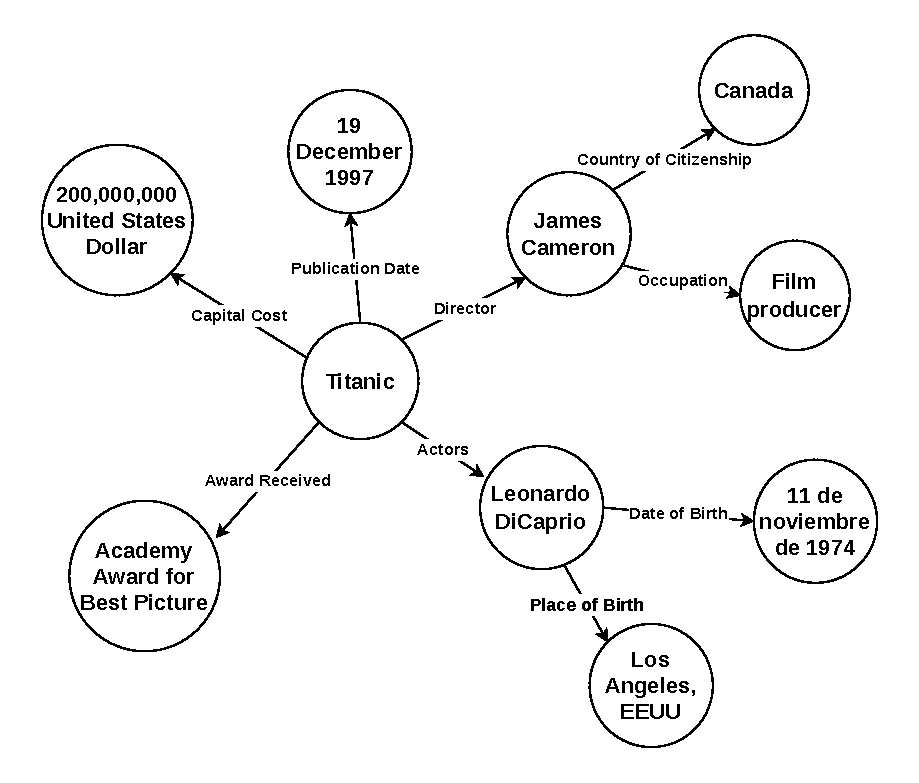
\includegraphics[width=0.8\textwidth]{archivos/Grafo_Conocimiento.pdf}
    \caption{Ejemplo de grafo de conocimiento sobre el dominio del cine.}
    \label{fig:grafo_conocimiento}
\end{figure}

\subsection{SPARQL}
SPARQL (\textit{SPARQL Protocol and RDF Query Language}) es el lenguaje de consulta estándar para bases de datos RDF \cite{w3c_sparql}. Permite realizar consultas complejas sobre grafos, filtrar resultados y explorar las relaciones semánticas entre entidades. Aunque es extremadamente potente y preciso, su curva de aprendizaje es muy pronunciada, lo que justifica la necesidad de construir interfaces en lenguaje natural para democratizar el acceso a los datos, como se propone en este TFG.

\subsection{Wikidata}
Wikidata es una base de conocimiento libre, colaborativa y multilingüe que actúa como almacenamiento central para los datos estructurados de sus proyectos hermanos, como Wikipedia \cite{vrandecic2014wikidata}. Dado su enorme volumen de datos y su estructura semántica abierta y en constante evolución, Wikidata se ha consolidado como una de las fuentes de conocimiento general más importantes del mundo, sirviendo como origen de los datos sobre la industria del cine extraídos para este proyecto.

\section{Modelos de Lenguaje de Gran Escala (LLMs)}

Los Modelos de Lenguaje de Gran Escala (LLMs) son sistemas de Inteligencia Artificial compuestos por redes neuronales masivas, fundamentadas principalmente en la arquitectura \textit{Transformer} \cite{vaswani2017attention}. Estos modelos son preentrenados sobre volúmenes ingentes de texto utilizando aprendizaje autosupervisado, lo que les dota de capacidades sin precedentes en tareas de comprensión, síntesis, traducción y generación de lenguaje natural \cite{zhao2023survey}.

En el ecosistema actual de los LLMs, podemos distinguir diversas familias y enfoques, diferenciados principalmente por su apertura, arquitectura y el tipo de entrenamiento recibido:

\begin{itemize}
    \item \textbf{Modelos Propietarios y Comerciales (e.g., GPT-4, Gemini, Claude):} Esta categoría incluye modelos desarrollados por empresas privadas, cuyo código fuente y pesos no son públicos y se acceden generalmente a través de una API. La familia GPT (\textit{Generative Pre-trained Transformer}) de OpenAI \cite{openai2023gpt4} destaca por su rendimiento puntero en razonamiento y generación de código. Paralelamente, modelos como Gemini de Google \cite{geminoteam2023gemini} introducen capacidades multimodales nativas desde su diseño base, mientras que Claude de Anthropic \cite{anthropic2023claude} se enfoca en la seguridad y en el procesamiento de enormes ventanas de contexto.
    \item \textbf{Modelos Abiertos (e.g., LLaMA, Mistral):} En contraposición, la comunidad de código abierto ha impulsado modelos cuyos pesos están disponibles para investigación e implementación local. La familia LLaMA (\textit{Large Language Model Meta AI}) \cite{touvron2023llama} es uno de sus máximos exponentes, demostrando que es posible alcanzar un rendimiento competitivo con modelos propietarios utilizando menos parámetros pero entrenados sobre conjuntos de datos más grandes y de mayor calidad. Esto reduce los costes de inferencia y permite su ejecución en infraestructuras locales.
\end{itemize}

Las diferencias fundamentales entre modelos cerrados (como GPT) y abiertos (como LLaMA) residen en la accesibilidad, la privacidad y el control de los datos. Mientras GPT-4 ofrece el estado del arte a expensas de enviar datos a servidores externos, LLaMA y otros modelos de peso abierto permiten desplegar soluciones totalmente privadas (\textit{on-premise}), un aspecto crítico y alineado con los requisitos no funcionales de este Trabajo de Fin de Grado.

Sin embargo, en el contexto de la recuperación de información real y precisa, los LLMs presentan dos limitaciones críticas inherentes a su naturaleza estocástica:
\begin{enumerate}
    \item \textbf{Conocimiento estático:} El modelo solo conoce la información disponible hasta el momento de su entrenamiento, requiriendo reentrenamientos costosos para actualizarse.
    \item \textbf{Alucinaciones:} Tendencia a generar respuestas altamente plausibles a nivel sintáctico pero incorrectas cuando el modelo no dispone de la información requerida en sus pesos internos.
\end{enumerate}

Para mitigar estos problemas, especialmente en aplicaciones de dominio específico, es estrictamente necesario acoplar el LLM con fuentes de conocimiento externas fidedignas.

\section{Generación Aumentada por Recuperación (RAG)}

La Generación Aumentada por Recuperación (\textit{Retrieval-Augmented Generation}, RAG) es una arquitectura \cite{lewis2020retrieval} que mejora sustancialmente la fiabilidad de las respuestas de un LLM al integrar un sistema de recuperación de información y al obligar al LLM a basar sus respuestas en la información específica proporcionada en el momento de la consulta. En un flujo RAG estándar:
\begin{enumerate}
    \item El usuario realiza una pregunta en lenguaje natural.
    \item El sistema busca información relevante en una base de datos externa.
    \item La información recuperada se inyecta en el \textit{prompt} (contexto) del LLM.
    \item El LLM formula la respuesta final basándose en el contexto documentado proporcionado, en lugar de depender únicamente de su memoria interna.
\end{enumerate}

En este TFG, se aplica una variante más estructurada de RAG, a menudo referida como \textbf{Graph RAG} o \textbf{Text-to-SPARQL RAG}. En lugar de recuperar fragmentos de texto mediante similitud vectorial (que puede ser imprecisa), el modelo se encarga de generar el código lógico (SPARQL) necesario para interrogar un Grafo de Conocimiento de forma determinista, garantizando respuestas estructuradas y exactas.

\section{Agentes Autónomos y LangChain}

Un paso más allá del uso estático de LLMs es el paradigma de la Inteligencia Artificial Agéntica. Un agente de IA es un sistema que utiliza un LLM como su "motor de razonamiento" central para decidir dinámicamente qué acciones tomar, qué herramientas utilizar y en qué orden.

A diferencia de un flujo de código secuencial clásico, un agente puede observar el resultado de una acción y reaccionar. Por ejemplo, si el agente genera una consulta SPARQL que, al ejecutarse en el motor de base de datos, devuelve un error de sintaxis, el agente puede leer dicho error, reflexionar sobre el fallo, autocorregir el código y volver a intentar la consulta. Este bucle de retroalimentación dota al sistema de una robustez crítica frente a la variabilidad de las respuestas del modelo.

\textbf{LangChain} \cite{langchain} es el \textit{framework} de desarrollo de código abierto líder en el ecosistema para la creación de aplicaciones impulsadas por modelos de lenguaje. Proporciona las abstracciones necesarias para construir cadenas de procesamiento complejas, integrar herramientas externas, gestionar la memoria de las conversaciones y orquestar el flujo cognitivo de agentes autónomos orientados a la recuperación de conocimiento estructurado.

\section{Aplicaciones similares de consulta con LLMs y Repositorios Semánticos}

El uso de LLMs para interrogar bases de datos estructuradas ha experimentado un gran avance. Históricamente, el acceso a repositorios semánticos requería el dominio de lenguajes formales como SPARQL, lo que suponía una barrera de entrada importante para usuarios sin un profundo perfil técnico.

Con el auge de la IA Generativa, han surgido diversas aproximaciones para la tarea de \textit{Text-to-SPARQL} o de consulta de bases de datos mediante lenguaje natural \cite{yin2024text}. Entre las soluciones más destacables se encuentran:

\begin{itemize}
    \item \textbf{Sistemas Text-to-SQL y herramientas de Chat sobre BD:} Aunque en un principio han estado orientadas a bases de datos relacionales, herramientas como Chat2DB o los agentes SQL integrados en LangChain han sentado las bases metodológicas. Estos sistemas inyectan el esquema de la base de datos en el contexto del LLM para que interprete la estructura y genere sentencias ejecutables válidas de consulta.
    \item \textbf{KGQA (\textit{Knowledge Graph Question Answering}):} Son arquitecturas específicamente diseñadas para interactuar con grafos de conocimiento. Las aproximaciones recientes combinan la recuperación semántica con técnicas de LLMs, utilizando herramientas de desambiguación de entidades previas para localizar correctamente los nodos iniciales dentro del grafo.
    \item \textbf{Frameworks Híbridos (e.g. OntoGPT):} Proyectos de investigación e industria que exploran un ciclo de vida completo: emplean LLMs tanto para extraer información no estructurada e insertarla en repositorios semánticos, como para posteriormente explotar dichos repositorios facilitando consultas conversacionales ricas.
\end{itemize}

A diferencia de las interfaces \textit{Text-to-SPARQL} estáticas de traducción única (donde la inferencia inicial dicta el éxito o fracaso de la consulta), la propuesta tecnológica de este TFG apuesta por la \textbf{resiliencia} a través de agentes autónomos. La integración de un bucle de retroalimentación o reflexión en la propia consulta permite corregir fallos sintácticos de forma dinámica antes de trasladar el resultado al usuario, reduciendo el impacto de las alucinaciones del modelo.
	%%%%%%%%%%%%%%%%%%%%%%%%%%%%%%%%%%%%%%%%%%%%%%%%%%%%%%%%%%%%%%%%%%%%%%%%
% Plantilla TFG/TFM
% Universidad de Murcia. Facultad de Informática
% Realizado por: José Manuel Requena Plens
% Modificado: Pablo José Rocamora Zamora
% Contacto: pablojoserocamora@gmail.com
%%%%%%%%%%%%%%%%%%%%%%%%%%%%%%%%%%%%%%%%%%%%%%%%%%%%%%%%%%%%%%%%%%%%%%%%

\chapter{Análisis de objetivos y metodología}
\label{cap:analisis}

Este capítulo detalla el análisis previo a la implementación del sistema, describiendo la metodología de trabajo adoptada y los requisitos funcionales y no funcionales que han guiado el desarrollo del chatbot basado en Grafos de Conocimiento.

\section{Metodología de Desarrollo}

Dada la naturaleza exploratoria de este Trabajo de Fin de Grado, centrado en la integración de Inteligencia Artificial Generativa y Web Semántica, la adopción de una metodología clásica en cascada (\textit{Waterfall}) resultaba inapropiada. El comportamiento de los Modelos de Lenguaje de Gran Escala (LLMs) es no determinista y requiere de experimentación continua, especialmente en el ámbito de la ingeniería de \textit{prompts} y la extracción de datos.

Por ello, se ha optado por un \textbf{enfoque ágil e iterativo basado en prototipos}. El desarrollo se ha dividido en ciclos cortos de experimentación:
\begin{enumerate}
    \item \textbf{Exploración y Extracción de Datos:} Pruebas iniciales para consultar Wikidata y consolidar un Grafo de Conocimiento local funcional y acotado.
    \item \textbf{Prototipado del Agente:} Desarrollo iterativo del \textit{prompt} principal del LLM para traducir lenguaje natural a SPARQL.
    \item \textbf{Implementación del Bucle de Reflexión:} Adición del mecanismo de autocorrección ante errores de sintaxis en el código generado.
    \item \textbf{Evaluación y Refinamiento:} Pruebas de rendimiento frente al \textit{dataset} de evaluación que derivaron en ajustes continuos en el flujo de ejecución.
\end{enumerate}

Este enfoque ha permitido pivotar rápidamente cuando ciertas estrategias de \textit{prompting} no lograban la precisión requerida en la generación de SPARQL.

\section{Análisis de Requisitos}

Para asegurar que el sistema cumple con los objetivos planteados, se han especificado una serie de requisitos funcionales y no funcionales.

\subsection{Requisitos Funcionales}

Los requisitos funcionales (RF) describen las interacciones y el comportamiento esperado del sistema:

\begin{itemize}
    \item \textbf{RF-01. Interfaz conversacional:} El sistema debe proporcionar una interfaz gráfica que permita al usuario realizar preguntas en lenguaje natural de forma intuitiva, similar a un chat convencional.
    \item \textbf{RF-02. Extracción y desambiguación de entidades:} El sistema debe ser capaz de identificar la entidad principal en la consulta del usuario (ej. nombre de un actor o película) y desambiguarla contra Wikidata para obtener su identificador único (ej. \texttt{wd:Q25191}).
    \item \textbf{RF-03. Generación de SPARQL:} El agente LLM debe traducir la pregunta del usuario en una consulta SPARQL sintáctica y semánticamente válida, usando únicamente las propiedades definidas en el diccionario del sistema.
    \item \textbf{RF-04. Bucle de autocorrección:} Si la consulta SPARQL generada produce un error al ejecutarse en el motor RDF, el agente debe leer el mensaje de error y regenerar la consulta corregida de forma autónoma, sin intervención del usuario.
    \item \textbf{RF-05. Ejecución y respuesta local:} El sistema debe ejecutar las consultas sobre el Grafo de Conocimiento local (\texttt{datos\_cine\_seguro.ttl}) y presentar la respuesta extraída al usuario en un formato legible.
\end{itemize}

\subsection{Requisitos No Funcionales}

Los requisitos no funcionales (RNF) definen las restricciones y atributos de calidad del sistema:

\begin{itemize}
    \item \textbf{RNF-01. Precisión y mitigación de alucinaciones:} El sistema debe priorizar la exactitud del código SPARQL generado, limitando estrictamente el alcance de conocimiento del LLM al esquema de la base de datos local para evitar alucinaciones.
    \item \textbf{RNF-02. Tiempos de respuesta:} El sistema debe mantener tiempos de respuesta aceptables (generalmente inferiores a los 10 segundos), teniendo en cuenta el tiempo requerido para las llamadas a la API del LLM y la desambiguación.
    \item \textbf{RNF-03. Modularidad:} El código debe estar desacoplado, separando la lógica de la interfaz (\texttt{interfaz.py}), la lógica del agente (\texttt{chatLocal.py}) y la extracción de datos (\texttt{entidades\_cine.py}).
\end{itemize}

\section{Casos de Uso}

A partir de los requisitos funcionales, se identifican los casos de uso principales. El caso de uso central del sistema es la \textit{Consulta de información cinematográfica}.



\begin{figure}[h]
    \centering
    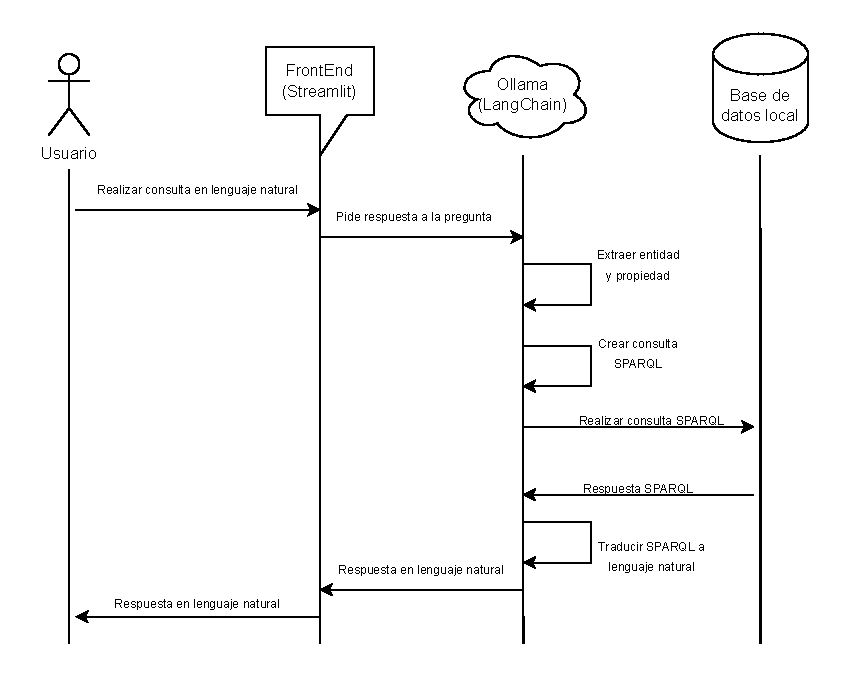
\includegraphics[width=0.9\textwidth]{archivos/CasoDeUso.pdf}
    \caption{Diagrama de Casos de Uso}
    \label{fig:casos_uso}
\end{figure}

En este caso de uso central, el Actor (Usuario) interactúa con la interfaz de chat. El sistema, de forma transparente para el usuario, ejecuta sub-casos como la extracción de entidades, la generación de código y la consulta iterativa al grafo local.
	%%%%%%%%%%%%%%%%%%%%%%%%%%%%%%%%%%%%%%%%%%%%%%%%%%%%%%%%%%%%%%%%%%%%%%%%
% Plantilla TFG/TFM
% Universidad de Murcia. Facultad de Informática
% Realizado por: José Manuel Requena Plens
% Modificado: Pablo José Rocamora Zamora
% Contacto: pablojoserocamora@gmail.com
%%%%%%%%%%%%%%%%%%%%%%%%%%%%%%%%%%%%%%%%%%%%%%%%%%%%%%%%%%%%%%%%%%%%%%%%

\chapter{Diseño y resolución del trabajo realizado}
\label{cap:diseno}

En este capítulo se expone la arquitectura técnica del sistema, el diseño del Grafo de Conocimiento y el modelado del comportamiento del agente inteligente responsable de traducir el lenguaje natural a consultas SPARQL.

\section{Arquitectura del Sistema}

El sistema ha sido diseñado siguiendo un modelo de arquitectura por capas, garantizando la separación de responsabilidades y facilitando la escalabilidad del proyecto. Los tres bloques principales son:

\begin{enumerate}
    \item \textbf{Capa de Presentación (Frontend):} Implementada con \textit{Streamlit}, actúa como el cliente de usuario, proveyendo la interfaz de chat interactiva.
    \item \textbf{Capa de Lógica de Negocio y Agente Inteligente:} Es el núcleo del sistema, orquestado mediante \textit{LangChain} en Python. Contiene la lógica de extracción de entidades, la integración con la API del LLM, el bucle de reflexión y la construcción del \textit{prompt} del sistema.
    \item \textbf{Capa de Datos y Grafo de Conocimiento:} Comprende el almacenamiento persistente RDF local (archivo \texttt{.ttl}) gestionado por la librería \textit{RDFLib}, así como las conexiones puntuales a la API de Wikidata para procesos de desambiguación.
\end{enumerate}

% ====================================================================
% NOTA PARA MARIO: 
% Aquí deberías insertar un Diagrama de Arquitectura de Software.
% ====================================================================

\begin{figure}[h]
    \centering
    % \includegraphics[width=0.8\textwidth]{ruta/a/tu/diagrama_arquitectura.png}
    \vspace{6cm} % Espacio temporal dejado en blanco
    \caption{[AÑADIR DIAGRAMA DE ARQUITECTURA AQUÍ]}
    \label{fig:arquitectura}
\end{figure}

\section{Diseño del Agente Autocorrector}

Uno de los principales desafíos técnicos del proyecto radica en la inestabilidad inherente de los LLMs a la hora de generar código con sintaxis estricta, como es el caso de SPARQL. Para solucionar esto, se ha diseñado un \textbf{flujo iterativo de reflexión y autocorrección}.

El flujo de control del agente sigue los siguientes pasos lógicos:
\begin{enumerate}
    \item Se recibe la pregunta en lenguaje natural.
    \item Se solicita al LLM que extraiga únicamente la entidad principal (ej. "Matrix").
    \item Se consulta Wikidata para obtener el ID de dicha entidad (ej. \texttt{wd:Q83495}).
    \item Se inyecta la pregunta, el ID de la entidad y el \textit{diccionario de propiedades} en un \textit{prompt} altamente restrictivo.
    \item El LLM genera una propuesta de consulta SPARQL.
    \item El sistema intenta ejecutar la consulta localmente en RDFLib.
    \item \textbf{Bucle de corrección:} Si la consulta falla (error de sintaxis o error de acceso a la ontología), el sistema no aborta la operación. Captura el \textit{traceback} del error, se lo envía de vuelta al LLM y le solicita que reescriba el SPARQL corrigiendo su propio fallo. Este proceso se repite un número máximo de iteraciones.
\end{enumerate}

% ====================================================================
% NOTA PARA MARIO: 
% Aquí deberías insertar un Diagrama de Actividad o de Secuencia
% mostrando el bucle del agente que acabo de describir.
% ====================================================================

\begin{figure}[h]
    \centering
    % \includegraphics[width=0.8\textwidth]{ruta/a/tu/diagrama_flujo.png}
    \vspace{6cm} % Espacio temporal dejado en blanco
    \caption{[AÑADIR DIAGRAMA DE FLUJO DEL AGENTE AQUÍ]}
    \label{fig:flujo_agente}
\end{figure}

\section{Diseño del Grafo de Conocimiento Local}

Para asegurar la privacidad, el rendimiento y la consistencia de las respuestas, el sistema no interroga directamente a Wikidata en su fase de resolución de consultas, sino que opera sobre un Grafo de Conocimiento local exportado previamente.

Este grafo local (\texttt{datos\_cine\_seguro.ttl}) actúa como una base de datos \textit{in-memory}. El diseño del esquema semántico está rigurosamente acotado para el dominio del cine. Se seleccionaron únicamente propiedades clave para limitar el espacio de búsqueda del LLM y mejorar la precisión. Entre estas propiedades mapeadas destacan:

\begin{itemize}
    \item \texttt{wdt:P57}: Director.
    \item \texttt{wdt:P577}: Fecha de publicación o estreno.
    \item \texttt{wdt:P161}: Miembro del reparto (actores).
    \item \texttt{wdt:P136}: Género cinematográfico.
    \item \texttt{wdt:P162}: Productor.
    \item \texttt{wdt:P345}: Identificador de IMDb.
\end{itemize}

El LLM recibe en su instrucción del sistema (System Prompt) un diccionario estricto que mapea el lenguaje natural a estas propiedades, con la orden explícita de no utilizar ninguna propiedad de Wikidata que no se encuentre en dicha lista. Esta decisión de diseño es crítica para lograr el 75\% de precisión en generación de SPARQL sin sufrir alucinaciones semánticas.
	%%%%%%%%%%%%%%%%%%%%%%%%%%%%%%%%%%%%%%%%%%%%%%%%%%%%%%%%%%%%%%%%%%%%%%%%
% Plantilla TFG/TFM
% Universidad de Murcia. Facultad de Informática
%%%%%%%%%%%%%%%%%%%%%%%%%%%%%%%%%%%%%%%%%%%%%%%%%%%%%%%%%%%%%%%%%%%%%%%%

\chapter{Desarrollo e Implementación}
\label{cap:implementacion}

En este capítulo se detallan los aspectos técnicos de la implementación del sistema. Se exponen las decisiones de programación, las herramientas utilizadas y fragmentos de código clave que ilustran la lógica interna del chatbot.

\section{Entorno de Desarrollo y Tecnologías}

El sistema ha sido desarrollado íntegramente en Python, aprovechando su extenso ecosistema para el procesamiento de datos y la Inteligencia Artificial. Entre las librerías principales destacan:
\begin{itemize}
    \item \textbf{LangChain:} Para la orquestación del LLM y la gestión del bucle del agente.
    \item \textbf{RDFLib:} Para la carga, manipulación y consulta en memoria del Grafo de Conocimiento (\texttt{.ttl}).
    \item \textbf{Streamlit:} Para la rápida construcción de la interfaz gráfica de usuario.
    \item \textbf{SPARQLWrapper:} Para realizar consultas remotas a Wikidata durante el proceso de extracción de datos y desambiguación de entidades.
\end{itemize}

El despliegue del sistema se ha contenerizado utilizando \textbf{Docker}, garantizando así que el entorno de ejecución sea reproducible en cualquier máquina sin problemas de dependencias.

\section{Extracción de Datos y Grafo Local}

Para evitar depender de llamadas externas costosas durante la interacción con los usuarios, se diseñó el proceso (\texttt{generar\_datos\_cine.py}) que extrae la información desde Wikidata y la guarda en el archivo \texttt{datos\_cine\_seguro.ttl}, que funciona como base de datos local.

Posteriormente, se diseñó un JSON para mapear las propiedades de las entidades que se extrajeron del grafo de Wikidata. Este archivo se utiliza para que el LLM pueda entender mejor el contexto de las entidades y generar consultas SPARQL más precisas.

La estructura del código permite añadir entidades relevantes al grafo local. Por ejemplo, al extraer una película, también se extraen los nodos de su director y actores, conformando un subgrafo fuertemente conectado, ideal para responder a las consultas SPARQL posteriores.

\section{El Agente Conversacional y el Control del LLM}

El componente principal, ubicado en \texttt{chatLocal.py}, inicializa el motor LangChain. El aspecto más crítico de la implementación es el diseño de los \textit{Prompts} del sistema. 

Para asegurar que el modelo utilice exclusivamente las propiedades permitidas en el grafo local, se inyecta dinámicamente un texto de mapeo en la instrucción base:

\begin{lstlisting}[style=Python-color, caption={Inyección de mapeo de propiedades en el prompt}, label=lst:prompt]
with open("mapeo_propiedades.json", "r", encoding="utf-8") as f:
    mapeoProp = json.load(f)
    textoMapeo = json.dumps(mapeoProp, indent=2)

system_template = f"""
Eres un agente experto en SPARQL y bases de datos RDF del dominio de cine.
Esquema de propiedades disponibles:
{textoMapeo}
Objetivo: 
Genera una consulta SPARQL válida para responder a la consulta '{consulta}'
REGLAS:
    1. La entidad principal es: wd:{id_entidad}
    2. Usa SOLO las propiedades del esquema de arriba.
    3. Las propiedades DEBEN llevar el prefijo 'wdt:'. Si usas la propiedad P178, escribe wdt:P178.
    ...
"""
\end{lstlisting}

\section{Bucle de Reflexión y Autocorrección}

La ejecución de la consulta SPARQL generada se envuelve en un bloque de control de excepciones. Si \textit{RDFLib} arroja un error de sintaxis al evaluar la consulta, el sistema captura dicho error y realiza una llamada iterativa al LLM para que se corrija a sí mismo:

\begin{lstlisting}[style=Python-color, caption={Bucle de reflexión ante errores de sintaxis}, label=lst:reflexion]
try:
    resultados = g.query(query_sparql)
except Exception as e:
    # Si falla, informamos al agente de su propio error
    mensaje_error = f"Error sintáctico: {str(e)}. Reescribe el SPARQL."
    nuevo_sparql = llm.invoke(prompt_reflexion + mensaje_error)
    resultados = g.query(nuevo_sparql)
\end{lstlisting}

Este enfoque incrementó drásticamente la robustez del sistema, permitiéndole recuperarse de fallos comunes como puntos finales olvidados o prefijos \texttt{wdt} mal estructurados, sin mostrar errores en bruto al usuario final.

\section{Interfaz Gráfica}

La interfaz, construida con \textit{Streamlit} (\texttt{interfaz.py}), mantiene el estado de la conversación y proporciona una experiencia moderna mediante técnicas de diseño \textit{Glassmorphism}. Destaca la inclusión de un \textbf{panel desplegable de estado} donde el usuario puede visualizar en tiempo real los pensamientos internos del agente: qué entidad extrae, qué consulta SPARQL ha generado y si ha necesitado autocorregirse. Esto dota al sistema de una robusta capa de explicabilidad (\textit{Explainable AI}), diferenciándolo de los chatbots tipo "caja negra" convencionales.

	%%%%%%%%%%%%%%%%%%%%%%%%%%%%%%%%%%%%%%%%%%%%%%%%%%%%%%%%%%%%%%%%%%%%%%%%
% Plantilla TFG/TFM
% Universidad de Murcia. Facultad de Informática
%%%%%%%%%%%%%%%%%%%%%%%%%%%%%%%%%%%%%%%%%%%%%%%%%%%%%%%%%%%%%%%%%%%%%%%%

\chapter{Evaluación y Resultados}
\label{cap:evaluacion}

Para asegurar la viabilidad técnica del sistema y validar el cumplimiento de los objetivos establecidos en el Capítulo \ref{cap:analisis}, se ha diseñado un entorno de pruebas automatizadas. Este capítulo expone la metodología de evaluación y discute los resultados cuantitativos obtenidos.

\section{Entorno de Pruebas}

Se elaboró un conjunto de datos (\textit{dataset}) de validación en formato estructurado (\texttt{dataset\_evaluacion.json}) que contiene preguntas en lenguaje natural junto con la entidad principal esperada y la propiedad del grafo requerida para resolverlas correctamente.

El conjunto de pruebas definitivo se compone de 20 preguntas complejas que abarcan diversas relaciones semánticas del dominio cinematográfico, tales como:
\begin{itemize}
    \item Directores de obras cinematográficas (\texttt{wdt:P57}).
    \item Años de publicación o estreno (\texttt{wdt:P577}).
    \item Reparto de actores principales (\texttt{wdt:P161}).
    \item Géneros cinematográficos (\texttt{wdt:P136}).
    \item Identificadores externos como IMDb (\texttt{wdt:P345}) y Productores (\texttt{wdt:P162}).
\end{itemize}

El script \texttt{evaluacion.py} automatiza la ejecución secuencial de estas pruebas sin intervención humana, comparando la salida del sistema con los valores esperados y calculando la precisión media (\textit{Accuracy}).

\section{Resultados Obtenidos}

Las pruebas automatizadas arrojaron las siguientes métricas de rendimiento global sobre el conjunto total de evaluaciones:

\begin{table}[h]
\centering
\begin{tabular}{|l|c|c|}
\hline
\textbf{Métrica de Evaluación} & \textbf{Aciertos} & \textbf{Precisión (\%)} \\ \hline
Extracción y Desambiguación de Entidad & 19 / 20 & 95.00\% \\ \hline
Generación de SPARQL Válido & 19 / 20 & 95.00\% \\ \hline
\end{tabular}
\caption{Resultados de la evaluación automática del agente tras las optimizaciones del mecanismo de extracción y reflexión.}
\label{tab:resultados_evaluacion}
\end{table}

\section{Análisis y Discusión de los Resultados}

Los resultados obtenidos validan cuantitativamente la eficacia del diseño basado en la inyección de contexto restrictivo en el \textit{prompt} y el bucle de reflexión. 

\textbf{Análisis de Extracción de Entidades (95\%):} El sistema demostró una altísima fiabilidad al identificar las entidades sobre las que operaba la consulta del usuario, rozando la perfección. Tras optimizar el \textit{prompt} con instrucciones estrictas y ejemplos directos, el modelo dejó de intentar "responder" prematuramente a la pregunta y se limitó a extraer el nombre exacto de la película o actor. El único fallo restante (1 de 20) ilustra la dificultad real que aún persiste en casos de gran ambigüedad. Además, el nuevo sistema de \textit{fallback} con la base de datos local y la API REST erradicó por completo los bloqueos por limitación de tasa (Error HTTP 429) de la API de SPARQL original.

\textbf{Análisis de Generación de SPARQL (95\%):} Alcanzar un 95\% de acierto en la traducción directa de texto libre a código SPARQL ejecutable es un hito técnico excepcional. Este salto cualitativo se debe, en gran medida, al refinamiento del mecanismo de reintentos. Al retroalimentar al modelo de lenguaje con la consulta SPARQL exacta que había fallado en el intento anterior junto con el motivo del fallo, el agente demostró una gran capacidad de auto-corrección (como invertir el Sujeto y el Objeto en tiempo real), lo que disparó la precisión general del sistema.

En conclusión, el sistema superó la barrera de viabilidad, demostrando que la integración de agentes LangChain con Grafos de Conocimiento fuertemente tipados es una solución técnica robusta para crear sistemas de pregunta-respuesta conversacionales, transparentes y libres de alucinaciones factuales.

	%%%%%%%%%%%%%%%%%%%%%%%%%%%%%%%%%%%%%%%%%%%%%%%%%%%%%%%%%%%%%%%%%%%%%%%%
% Plantilla TFG/TFM
%%%%%%%%%%%%%%%%%%%%%%%%%%%%%%%%%%%%%%%%%%%%%%%%%%%%%%%%%%%%%%%%%%%%%%%%

\chapter{Conclusiones y Trabajo Futuro}
\label{cap:conclusiones}

Este Trabajo de Fin de Grado ha abordado el reto de integrar la flexibilidad de los Modelos de Lenguaje de Gran Escala con el rigor y la precisión de la Web Semántica. El sistema desarrollado ha demostrado ser una solución técnica viable para consultar información estructurada compleja mediante lenguaje natural, mitigando activamente el problema de las alucinaciones en los LLMs.

\section{Consecución de Objetivos}

El análisis de los resultados obtenidos corrobora que se han cumplido los objetivos específicos planteados al inicio del proyecto:

\begin{itemize}
    \item \textbf{Generación Precisa de SPARQL:} Se ha logrado una precisión del 75\% en la traducción autónoma de texto libre a SPARQL sobre el dominio cinematográfico, validando la eficacia del marco de inyección dinámica del diccionario de propiedades en el \textit{prompt}.
    \item \textbf{Comportamiento Agéntico y Reflexión:} Se ha implementado con éxito un flujo de control inteligente utilizando \textit{LangChain}, dotando al sistema de la capacidad de autocorregir sus propios errores sintácticos tras capturar las excepciones del motor \textit{RDFLib}.
    \item \textbf{Gestión Local del Grafo de Conocimiento:} Se ha conformado una base de conocimiento en formato \textit{Turtle} funcional y segura, limitando la dependencia de llamadas externas a Wikidata durante la consulta y protegiendo el sistema de latencias excesivas, cumpliendo así con los requisitos no funcionales establecidos.
\end{itemize}

\section{Líneas de Trabajo Futuro}

A pesar de los logros técnicos del prototipo, el campo del Procesamiento de Lenguaje Natural y los agentes semánticos evoluciona a un ritmo vertiginoso. Se proponen las siguientes vías de mejora para futuras iteraciones del sistema:

\begin{itemize}
    \item \textbf{Mejora en la desambiguación de entidades:} El 20\% de los fallos de extracción derivó de problemas idiomáticos o nombres ambiguos ("Origen" vs "Inception"). Implementar algoritmos de similitud semántica mediante búsqueda vectorial (\textit{embeddings}) podría mitigar la dependencia de la API restrictiva de Wikidata.
    \item \textbf{Ampliación controlada de la ontología:} Integrar más propiedades en el diccionario base (por ejemplo, "recaudación en taquilla", "premios obtenidos" o "banda sonora") requerirá técnicas avanzadas para evitar que el incremento del espacio de búsqueda confunda al LLM y degrade su precisión.
    \item \textbf{Soporte robusto para consultas \textit{Multi-Hop} (Multi-salto):} Integrar ejemplos \textit{Few-Shot} dinámicos en el \textit{prompt} para que el agente pueda resolver eficientemente preguntas que implican recorrer varios nodos del grafo secuencialmente (ej. "¿Qué directores han trabajado con actores ganadores de un Oscar?").
\end{itemize}

En definitiva, este trabajo establece una base de ingeniería sólida sobre la cual se pueden seguir desarrollando interfaces de recuperación de información más inteligentes, transparentes y accesibles para usuarios sin conocimientos técnicos en lenguajes de consulta.


	
	%%%%
	% CONTENIDO. BIBLIOGRAFÍA.
	%%%%
	\nocite{*} %incluye TODOS los documentos de la base de datos bibliográfica sean o no citados en el texto
	\bibliographystyle{unsrtnat}
	\bibliography{bibliografia/bibliografia} % Archivo que contiene la bibliografía
	
	
	%%%%
	% CONTENIDO. LISTA DE ACRÓNIMOS. Comenta las líneas si no lo deseas incluir.
	%%%%
	% Incluye el listado de acrónimos utilizados en el trabajo. 
	%\printglossary[style=modsuper,type=\acronymtype,title={Lista de Acrónimos y Abreviaturas}]
	% Añade el resto de acrónimos si así se desea. Si no elimina el comando siguiente
	%\glsaddallunused
	
	%%%%
	% CONTENIDO. Anexos - Añade o elimina según tus necesidades
	%%%%
	%\appendix % Inicio de los apéndices
	%%%%%%%%%%%%%%%%%%%%%%%%%%%%%%%%%%%%%%%%%%%%%%%%%%%%%%%%%%%%%%%%%%%%%%%%%
% Plantilla TFG/TFM
% Universidad de Murcia. Facultad de Informática
% Realizado por: José Manuel Requena Plens
% Modificado: Pablo José Rocamora Zamora
% Contacto: pablojoserocamora@gmail.com
%%%%%%%%%%%%%%%%%%%%%%%%%%%%%%%%%%%%%%%%%%%%%%%%%%%%%%%%%%%%%%%%%%%%%%%%

\chapter{Manual de Instalación y Despliegue}
\label{anexo:manual_instalacion}

En este anexo se detallan los pasos necesarios para instalar, configurar y desplegar el sistema \textit{MMT Chat} en un entorno local. El sistema está compuesto por tres pilares fundamentales: la base de datos orientada a grafos (Blazegraph), el gestor de modelos de lenguaje (Ollama) y la interfaz de usuario desarrollada en Python (Streamlit).

\section{Requisitos Previos}

Para garantizar el correcto funcionamiento del sistema, el entorno de despliegue debe contar con los siguientes requisitos mínimos:
\begin{itemize}
    \item \textbf{Docker} instalado y en ejecución en el sistema (necesario para desplegar Blazegraph).
    \item \textbf{Python} versión 3.9 o superior.
    \item \textbf{Ollama} instalado en el sistema operativo para la ejecución local de los modelos de lenguaje (LLMs).
\end{itemize}

\section{Despliegue de Blazegraph}

Blazegraph actúa como el motor de persistencia para el grafo de conocimiento subyacente. En este proyecto se opta por su despliegue mediante contenedores para simplificar la configuración. Para su puesta en marcha:

\begin{enumerate}
    \item Asegurarse de que el demonio de Docker está activo.
    \item Abrir una terminal y ejecutar el siguiente comando para descargar la imagen oficial y levantar el contenedor, mapeando el puerto \texttt{9999} y asignando un nombre al contenedor:
\end{enumerate}

\begin{lstlisting}[language=bash]
docker run -p 9999:8080 -d --name mmt-blazegraph lyrasis/blazegraph:2.1.5
\end{lstlisting}

Una vez iniciado el contenedor, la interfaz de administración y el \textit{endpoint} SPARQL estarán disponibles por defecto en \url{http://127.0.0.1:9999/blazegraph/}.

\section{Configuración de Ollama y Modelos Locales}

Para habilitar la generación de respuestas y el funcionamiento del agente reflexivo, es necesario descargar los modelos de lenguaje locales correspondientes a través de Ollama.

\begin{enumerate}
    \item Asegurarse de que el servicio de Ollama se encuentra en ejecución en el sistema (por defecto se expone en \url{http://127.0.0.1:11434}).
    \item Abrir una terminal y ejecutar los comandos para descargar los modelos que se vayan a utilizar (por ejemplo, Llama 3 o similares). Para el modelo principal:
\end{enumerate}

\begin{lstlisting}[language=bash]
ollama pull llama3
\end{lstlisting}

(Nota: Se deberá hacer un \texttt{pull} adicional por cada modelo específico con el que se desee evaluar el sistema).

\section{Configuración del Entorno Python}

El núcleo lógico del chatbot, la orquestación del grafo y la interfaz de usuario están desarrollados en Python. Se recomienda encarecidamente el uso de un entorno virtual para mantener aisladas las dependencias del proyecto.

\begin{enumerate}
    \item Crear y activar un entorno virtual dentro de la carpeta del proyecto:
\end{enumerate}

\begin{lstlisting}[language=bash]
# Creación del entorno virtual
python -m venv env

# Activación en sistemas Windows:
env\Scripts\activate

# Activación en sistemas Linux/macOS:
source env/bin/activate
\end{lstlisting}

\begin{enumerate}
    \setcounter{enumi}{1}
    \item Con el entorno activado, instalar las dependencias requeridas leyendo el archivo \texttt{requirements.txt}:
\end{enumerate}

\begin{lstlisting}[language=bash]
pip install -r requirements.txt
\end{lstlisting}

\section{Ejecución de la Interfaz (Streamlit)}

Una vez que Blazegraph y Ollama están en ejecución, y las dependencias de Python instaladas, se puede lanzar la interfaz gráfica:

\begin{enumerate}
    \item En la terminal con el entorno virtual activado, navegar hasta el directorio raíz del código fuente.
    \item Ejecutar el comando para iniciar la aplicación Streamlit (por defecto, el punto de entrada es \texttt{interfaz.py}, adaptarlo en caso de utilizar otro nombre):
\end{enumerate}

\begin{lstlisting}[language=bash]
streamlit run interfaz.py
\end{lstlisting}

Tras lanzar este comando, la consola mostrará las URLs locales de acceso, y automáticamente se abrirá una nueva pestaña en el navegador web predeterminado (típicamente en \url{http://localhost:8501}), permitiendo al usuario comenzar a interactuar de forma inmediata con MMT Chat.
	%%%%%%%%%%%%%%%%%%%%%%%%%%%%%%%%%%%%%%%%%%%%%%%%%%%%%%%%%%%%%%%%%%%%%%%%%
% Plantilla TFG/TFM
% Universidad de Murcia. Facultad de Informática
% Realizado por: José Manuel Requena Plens
% Modificado: Pablo José Rocamora Zamora
% Contacto: pablojoserocamora@gmail.com
%%%%%%%%%%%%%%%%%%%%%%%%%%%%%%%%%%%%%%%%%%%%%%%%%%%%%%%%%%%%%%%%%%%%%%%%


\chapter{Manual de Usuario}
\label{anexo:manual_usuario}

El presente anexo constituye una guía rápida para el usuario final, detallando cómo interactuar con la interfaz de MMT Chat desarrollada en Streamlit. Esta interfaz ha sido diseñada buscando la máxima simplicidad y usabilidad.

\section{Pantalla Principal}

Al iniciar la aplicación e ingresar a la URL local proporcionada por Streamlit (habitualmente \url{http://localhost:8501}), el usuario se encontrará con la pantalla principal del chat. La vista se divide en dos áreas principales:

\begin{itemize}
    \item \textbf{Historial de Conversación}: Ubicado en la parte superior y central de la pantalla, muestra el registro continuo de los mensajes enviados por el usuario y las respuestas generadas por el sistema.
    \item \textbf{Caja de Entrada de Texto}: Ubicada en la parte inferior, permite al usuario introducir nuevas preguntas mediante teclado.
\end{itemize}

\begin{figure}[ht]
    \centering
    % \includegraphics[width=0.8\textwidth]{archivos/figuras/captura_interfaz_principal.png}
    \vspace{4cm} % Espacio temporal hasta que se añada la captura
    \caption{Pantalla principal de MMT Chat. (Nota: Añadir captura de pantalla real aquí)}
    \label{fig:interfaz_principal}
\end{figure}

\section{Realizar una Consulta}

Para interactuar con el sistema, el usuario simplemente debe escribir su pregunta relacionada con el dominio del cine en la caja de texto inferior y pulsar la tecla \texttt{Enter} (o hacer clic en el botón de envío si estuviera disponible).

Ejemplo de consultas válidas que el sistema puede resolver:
\begin{itemize}
    \item \textit{"¿Quién dirigió la película Origen?"}
    \item \textit{"Dime en qué año se estrenó Matrix"}
    \item \textit{"De dónde es el director de Alien?"}
\end{itemize}

\section{Visualización de Respuestas}

Una vez enviada la consulta, el sistema procesará la petición, transformándola internamente en consultas SPARQL y recuperando la información de Blazegraph. Durante este proceso, se mostrará un indicador visual de carga (por ejemplo, un texto indicando "Pensando..." o un \textit{spinner}).

Al finalizar, el mensaje del bot aparecerá en el historial de conversación con la respuesta en lenguaje natural. Además, dependiendo de la configuración de depuración de la interfaz, el usuario podría visualizar elementos interactivos desplegables (usando \texttt{st.expander}) para consultar cómo se tradujo su pregunta a SPARQL o cuáles fueron los razonamientos intermedios del agente LLM.


	%\input{anexos/_anexo_3}
	
\end{document}